\documentclass[11pt,a4paper,titlepage]{article}
 \oddsidemargin 0.2in 
 \evensidemargin 0.2in
 \textwidth 6.0in
\usepackage[utf8]{inputenc}
\usepackage[T1]{fontenc}
\usepackage{lmodern}
\usepackage[english]{babel}
\usepackage[tbtags]{amsmath}
\usepackage{wasysym}
\usepackage{amssymb}
\usepackage{graphicx}
\usepackage{epic}
\usepackage{eepic}
\usepackage{multicol}
\usepackage{fancyhdr}
\usepackage{float}
\usepackage{fancybox}
\usepackage{subfig}
\usepackage{endnotes}
\usepackage{natbib}		% REFERENCER FORMATERET SOM NATURVIDENSKAB
\usepackage{latexsym} 
% \usepackage{feynmf}		%Package for feynman diagrams.
\usepackage{axodraw4j} % Packages for JaxoDraw
\usepackage{pstricks}
\usepackage{color}

% % % % % % % % % % % % % % % % Bra-Ket % % % % % % % % % % % % % % % %

\newcommand{\ket}[1]{
  |#1 \rangle
}

\newcommand{\bra}[1]{
  \langle #1|
}

\newcommand{\braket}[2]{
  \langle #1|#2 \rangle
}

% % % % % % % % % % % % % % % % FIGURER % % % % % % % % % % % % % % % %
\newcommand{\includefigure}[4]{
\begin{figure}[htbp] \centering
		\includegraphics[scale=#2]{#3}
		\caption{\footnotesize #4}
		\label{#1}
\end{figure}
}
% % % % % % % % % % % % % % OPSKRIFT PAA EN FIGUR % % % % % % % % % % % %

%\includefigure{NAVN_PAA_FIGUREN}{FIGURENS STORRELSE (0-1)}{FILNAVN}{FIGURTEKST}

% % % % % % % % % % % % % % % REFERENCER % % % % % % % % % % % % % % %
\renewcommand\notesname{Referencer}
\numberwithin{equation}{section}

%----Different font in captions----
\newcommand{\captionfonts}{\small}

\makeatletter  % Allow the use of @ in command names
\long\def\@makecaption#1#2{%
  \vskip\abovecaptionskip
  \sbox\@tempboxa{{\captionfonts #1: #2}}%
  \ifdim \wd\@tempboxa >\hsize
    {\captionfonts #1: #2\par}
  \else
    \hbox to\hsize{\hfil\box\@tempboxa\hfil}%
  \fi
  \vskip\belowcaptionskip}
\makeatother   % Cancel the effect of \makeatletter
%------------Define Keys-------------

\makeindex

\parskip        =    1ex
\parindent      =    0em
\baselineskip   =    2ex

% % % % % % % % % %% % % % % FANCY SHIZZLE? % % % % % % % % % % % % % % %
\pagestyle{fancy} % with this we ensure that the chapter and section headings are in lowercase.
 
\renewcommand{\sectionmark}[1]{\markright{\thesection\ #1}} 
\fancyhf{} 				% delete current header and footer
\fancyhead[LE,RO]{\bfseries\thepage} 
\fancyhead[LO]{\bfseries\rightmark} 
\fancyhead[RE]{\bfseries\leftmark} 
\renewcommand{\headrulewidth}{0.5pt} 
\renewcommand{\footrulewidth}{0pt} 
\addtolength{\headheight}{0.5pt} 	% space for the rule 
\fancypagestyle{plain}{
\fancyhead{}				% get rid of headers on plain pages 
\renewcommand{\headrulewidth}{0pt} 	% and the line 
}

% % % % % % % % % % % % % % % BEGIN DOCUMENT % % % % % % % % % % % % % % %
\begin{document}
\title{Bachelor's Project\\Search for NCG in hadronic Z decays.}
\author{Andreas Skielboe og Julie Hougaard}
\date{\today}
\maketitle
\pagenumbering{roman}

% % % % % % % % % % % % % % % ABSTRACT % % % % % % % % % % % % % % % % % %
\begin{abstract}
In the following report we will explore the consequences of noncommutative geometry especially in relation to Z -> gg decays.
\end{abstract}

\clearpage
\tableofcontents
\clearpage

\pagenumbering{arabic}

%% \includeonly{secondfile} %% Selective including.

% % % % % % % % % % % % % % INTRODUCTION % % % % % % % % % % % % % % % %

\section{Introduction}
In describing fundamental physical phenomena, physicists make use of the concept of a particle representing a certain small-scale state (of the order $10^-15$ m) of the universe. Particles can interact with each other to annihilate or create new particles (or states). To account for this we use the concept of interactions. With these two concepts in hand we can go on and build mathematical frameworks based on experimental results and/or purely mathematical ideas, with the intend to extend our knowledge of the Universe and increase the predictive power and accuracy of the theories involved. Using this method physicists have been able to create an extensive theoretical framework with amazing predictive accuracy. This framework is commonly know as the Standard Model of particle physics, abbreviated SM.

Another accurate framework was developed in the beginning of the last century by german physicist Albert Einstein. This framework, describing gravity on large scales, is know as the General Theory of Relativity (GR). Together with the SM these two theories represent our best current knowledge\footnote{Henceforth when we write knowledge the reader may assume this is equivalent to the information available from being able to predict the time evolution of physical systems or states.} of the physical Universe at the very large and very small scales.

A lot of effort as been put in to unifying the encompassing physical theory of the large GR, with the theory of the s and the SM


% % % % % % % % % % % % % % % THEORY % % % % % % % % % % % % % % % % % % 

\section{Theory}
\subsection{Quantum field theory}
The particles and interactions of the SM are described in the language of quantum mechanics and quantum field theory.

\subsubsection{Principle of least action}
The action $\mathcal{S}$ is a functional\footnote{A functional is something that takes as its argument a function and returns a scalar.} related to the time evolution of a physical system. Namely the action is the change in phase of the wave function of the system. The Lagrangian is defined as the rate of change of the phase and given as

\begin{equation}
	\mathcal{S} = \int_{t_i \mathcal{P}}^{t_f} L \textrm{d}t,
\end{equation}

where we integrate over all intermediate states taken by the system evolving from time $t_i$ to $t_f$. The principle of least action then states that the actual path taken by the system is one that minimizes the action, or more precisely one where the action is stationary. In other words the variation of the line integral going from $t_i$ to $t_f$ is zero \cite{goldstein1959};

\begin{equation}
	\delta \mathcal{S} = \delta \int_{t_i}^{t_f} L \textrm{d}t = 0.
\end{equation}

Using Hamilton's principle, and knowing the Lagrangian of the system, one can derive the equations of motion.

\subsubsection{The path integral formalism}
In 1948 Richard Feynman presented his new formulation of non relativistic quantum mechanics, using what is known as the path integral formalism \cite{feynman1948sta}. The path integral takes into account all possible paths that a particle, or any other quantum mechanical system, going from a state $\ket{i}$ to a state $\ket{f}$ can take. This can be changes in position, momentum, energy or other intrinsic variables and is represented as an intermediate state of the system. Generally, and this is actually a central point in quantum mechanics, we are not interested in the path taken, but only in the fact that at some time $t_{i}$ the particle was in a state $\ket{i}$ and at some later time $t_{f}$ the particle is in a state $\ket{f}$. In order to arrive at this quantum probability-amplitude we must sum, or integrate, over the infinitely many paths, that the system can take to go from initial to final state. Doing this the amplitude is given as  
% \cite{richter_path_integrals}
\begin{equation} \label{eq:path}
	\bra{f} U(t_f,t_i) \ket{i} = \mathcal{N} \int \mathcal{D}x e^{i\mathcal{S}},
\end{equation}

where $\mathcal{N}$ is a constant of the system, $U$ is the time translation operator, $\mathcal{D}$ is an abbreviation given by the relation 

\begin{equation}
	\int \mathcal{D} x \equiv \lim_{N \to \infty} \int dx_1 \dots dx_N
\end{equation}

and the action $\mathcal{S}$ is related to the Lagrangian by the action principle, given in the 1-D case by

\begin{equation}
	\mathcal{S} = \int_{t_i}^{t_f} L(x,\dot{x},t)dt,
\end{equation}
where $x, \dot{x} \equiv \frac{dx}{dt}$ are generalized coordinates.

Equation \eqref{eq:path} is called the propagator in QFT. This equation describes the probability amplitude that a particle will go from the initial state to the final state in time $t_f - t_i$.

\subsubsection{Symmetry groups and gauge theories}
Noethe's Theorem states that for any transformation under which a physical system is invariant there exists a conserved quantity of that system. The classical examples are translations and rotations in the three spatial dimensions. If the system is invariant under those two transformations this corresponds to the conservation of linear and angular momentum. Thus these transformations forms a symmetry group of the theory. The two, physically equivalent situations, can be described by different mathematical configurations depending on the reference frame. The two descriptions are related to each other by this symmetry group.

In physics, any field theory in which the Lagrangian is invariant under some kind of continuous transformation is called a gauge theory, the invariance referred to as a gauge invariance. The group of transformations under which the Lagrangian is invariant is called the gauge group of the theory.\footnote{For a historical account of the development of gauge theories, at a level relevant for the present discussion, see \cite{gross1992gtp}.}

\subsubsection{Quantum electrodynamics and SU(1)}
In quantum mechanics the wave equation is invariant under local, space-time dependent, phase transformations, corresponding to rotations in the complex phase space of the wave function. In practice this invariance comes about when, in order to make predictions of physical observable, we have to take the absolute square of the wave function. Doing this information about the phase of the complex wave function is lost and we are left with only the absolute size of the complex number. This means that we can never physically measure the phase of the wave function, only its amplitude. Because of this, if we want the wave functions to represent actual physical systems, we have to insist that our equations be invariant under all local phase transformations\footnote{Actually the argument is a bit more subtle. There is no physical principle that states that the wavefunction \emph{has} to be invariant under local phase transformations, it is just something we assume. And, as it turns out, we can learn a lot from this assumption. \cite{griffiths1987iep}} of $\psi$ given by

\begin{equation} \label{eq:localphase}
    \psi \rightarrow e^{i\alpha(\mathbf{x})} \psi.
\end{equation}

Together these transformations form the mathematical symmetry group SU(1). This is simply the group of all transformations of the form \eqref{eq:localphase}.  So far this does not seem to pose any problems for us. Adding a phase may change the wave function, but all predictions made about the position of the particle, described by this function, are left invariant. Specifically

\begin{equation}
	|\psi|^2 \rightarrow |e^{i\alpha(\mathbf{x})} \psi|^2 = |\psi|^2.
\end{equation}

However for the derivative operator $\partial_\mu$ to be well-defined for all points in space-time we have to replace it by the covariant derivative

\begin{equation} \label{eq:covariant}
	\partial_\mu \rightarrow D_\mu = \partial_\mu - \textrm{i}e A_\mu.
\end{equation}

The covariant derivative compensates for the fact that, when making the local phase change, we pick up an extra factor of $i (\partial_\mu \theta)$ in the derivative of the Lagrangian. So we have introduced a new vector field $A_\mu$, designed to exactly cancel this extra factor, making sure that gauge invariance is satisfied under local continuous SU(1) transformations. The field, it turns out, is actually just the electromagnetic field know from classical theory of electromagnetism. When $A_\mu$ is quantized in the context of quantum field theory the quanta of this field are the photons, know as the gauge bosons of QED. By insistence on local gauge invariance of the Lagrangian of the free electron we get the electromagnetic field, and corresponding interactions, almost for free. This principle is the driving force behind the success of gauge theories.

\subsubsection{Gauging the SU(2) and SU(3) Lie groups}
The previous discussion outlines many of the essential principles of gauge theories. Following this logic the gauge group governing weak interaction turns out to be the composed group SU(1) $\times$ SU(2), where SU(2) is the group of $2 \times 2$ complex unitary matrices\footnote{More specifically SU(2) is a Lie group and its Lie algebra is the set of anti-Hermition $2 \times 2$ matrices with trace 0. For more information about Lie groups and Lie algebras see  \cite{fulton1991rtf}.}. Thus electromagnetism and the weak interaction responsible for radioactive decay are combined into one theory, the electroweak theory. The generators of SU(2) are the Pauli matrices

\begin{equation}
	\sigma_1 =
	\begin{pmatrix}
	0&1\\
	1&0
	\end{pmatrix},
	\sigma_2 = 
	\begin{pmatrix}
	0&-i\\
	i&0
	\end{pmatrix},
	\sigma_3 = 
	\begin{pmatrix}
	1&0\\
	0&-1
	\end{pmatrix}.
\end{equation}

The gauge boson associated with the weak force are the $W^+$, $W^-$ and the $Z^0$ bosons.

The gauge bosons mediating the strong interaction are characterized by the SU(3) gauge group. The generators of SU(3) are the 8 Gell-Mann matrices
\begin{align} \label{eq:gellmannmatrices}
	\lambda_1 &= \begin{pmatrix} 0 & 1 & 0 \\ 1 & 0 & 0 \\ 0 & 0 & 0 \end{pmatrix},
	\lambda_2 = \begin{pmatrix} 0 & -i & 0 \\ i & 0 & 0 \\ 0 & 0 & 0 \end{pmatrix},
	\lambda_3 = \begin{pmatrix} 1 & 0 & 0 \\ 0 & -1 & 0 \\ 0 & 0 & 0 \end{pmatrix},
	\lambda_4 = \begin{pmatrix} 0 & 0 & 1 \\ 0 & 0 & 0 \\ 1 & 0 & 0 \end{pmatrix}, \nonumber \\
	\lambda_5 &= \begin{pmatrix} 0 & 0 & -i \\ 0 & 0 & 0 \\ i & 0 & 0 \end{pmatrix},
	\lambda_6 = \begin{pmatrix} 0 & 0 & 0 \\ 0 & 0 & 1 \\ 0 & 1 & 0 \end{pmatrix},
	\lambda_7 = \begin{pmatrix} 0 & 0 & 0 \\ 0 & 0 & -i \\ 0 & i & 0 \end{pmatrix},
	\lambda_8 = \frac{1}{\sqrt{3}} \begin{pmatrix} 1 & 0 & 0 \\ 0 & 1 & 0 \\ 0 & 0 & -2 \end{pmatrix},
\end{align}

giving rise to 8 gauge bosons of the strong interaction know as gluons, each having a property called color. Because of this color feature the gauge theory of the strong interaction is called Quantum Chromodynamics (QCD). The reason for having 8 gluons is that we need 8 matrices to span the 'color' space laid out by the Gell-Mann matrices, while requiring that they have determinant 1. This is in fact the same reason why we need three Pauli matrices to span the group of SU(2) [KAN MAN SIGE DET, MATEMATISK?].

\subsection{The Standard Model}
Combining electroweak theory and quantum chromo dynamics using the group U(1) $\times$ SU(2) $\times$ SU(3) theorists are able to account for a great variety of elementary particles and interactions, and make profoundly accurate predictions. This theory is know as the Standard Model of particle physics. The Standard Model is a non abelian gauge theory. \footnote{Non abelian meaning that, save for U(1), the generators of the gauge groups are non-commuting.}

\subsubsection{Particles of the standard model}

% Billede med partikel-generationer fra Wikipedia.
\includefigure{fig:particle_generations}{0.3}{./images/particle_generations.eps}{The fundamental particles in the Standard Model. Fermions and bosons, listed in their respective generations. (Source: Wikimedia Commons).}

In the Standard Model of particle physics we divide the particles into two main groups; fermions and bosons. Fermions are defined as having half-integral spin and are described by Fermi-Dirac statistics, these include the leptons and quarks. Fermions constitutes all known matter and as such they are sometimes described as matter-particles. Bosons, on the other hand, have zero or integral spin and are described by Bose-Einstein statistics. Some of these, namely the gauge bosons, are responsible for the weak, strong and electromagnetic interactions. Therefore the gauge bosons are often called the force-carriers of their respective interactions. It may be appropriate to note that the formalism of quantum mechanics makes no clear distinction between the concepts of matter-particles and force-particles. Below is a table with all known quarks, leptons and gauge bosons. With the exception of neutrinos, which have to be detected in other ways, all of them have been seen in particle accelerator experiments.

\subsubsection{Feynman diagrams}
When calculating amplitudes for particle interactions in the SM it can be very instructive to make use of \emph{Feynman diagrams}. This approach was proposed by american physicist Richard P. Feynman in 1949 \cite{feynman1949sta}. A typical space-time interaction is the scattering of an electron and a positron by virtual annihalation followed by pair production. This process is represented as a Feynman diagram in Figure \ref{fig:feyn:ee_a_ee}. Space is extending top-down in the diagram while time is increasing from left to right. Arrows pointing along the flow of time, to the right, are particles, while arrows pointing against the flow of time, to the left, are anti-particles.

\begin{figure}[htp]
\centering
	\input{./jaxo/ee_a_ee_axis.tex}
\caption{Feynman diagram for the electromagnetic scattering of an electron and a positron. Time is increasing from left to right in the diagram.} \label{fig:feyn:ee_a_ee}
\end{figure}

The wavy line in the middle is a so called \emph{virtual particle}, in this case a virtual photon. It is virtual in the sense that we never actually measure it without disturbing the process and thereby destroying it. We can only ever measure the initial-state (incoming) particles and the final-state (outgoing) particles. Another reason why these, intermediate particles, are called virtual is suggested by looking at Figure \ref{fig:feyn:ee_a}. In the center-of-mass (CM) frame of the electron and positron, the two have exactly equal and opposite momenta. Together they have zero momentum in the CM-frame. Therefore the two particles can never annihilate to create a single photon, which always have momentum, given that it always travels at the speed $c$.

\begin{figure}[htp]
\centering
	\input{./jaxo/ee_a.tex}
\caption{Example of a virtual process in which an electron and a positron annihilates to crate a virtual photon seemingly violating conservation of momentum at the vertex. This process can never happen on its own, but it can form part of other diagrams in a similar way to that in Figure \ref{fig:feyn:ee_a_ee}.} \label{fig:feyn:ee_a}
\end{figure}

To uphold energy and momentum conservation at the vertex the virtual photon have to have an energy different from that of a free photon. In principle it can take on \emph{any} value. The virtual photon is said to be \emph{off mass shell} or simply \emph{off-shell}\footnote{See chapter 2 in \cite{griffiths1987iep} for more about virtual particles.}.

\subsubsection{Feynman rules and process amplitudes}
Using these diagrams Feynman were able to greatly simplify how we think about and calculate interactions in the SM. Having drawn a diagram as in Figure \ref{fig:feyn:ee_a_ee} we now want calculate the probability for this process to happen, that is to say we want the \emph{cross section} $\sigma$ of the process\footnote{See Appendix [DEN MED CROSS SECTIONS].}. Given the diagram one can write down the \emph{amplitude} $\mathcal{M}$ for this process, using so called \emph{Feynman rules} associated with the different parts of the diagram. Given $\mathcal{M}$ we can calculate the cross section using Fermi's Golden Rule. The amplitude, or the \emph{matrix element} at is is some times called, $\mathcal{M}$ accounts for the dynamics taking place in the interaction, while the Golden Rule, or \emph{phase space} factor, takes care of the kinematics.

To derive the actual feynman rules is way beyond this text, but we may still learn a lot by examining the results. Each vertex represents an interaction. Depending on the nature of this interaction we assign a number $g$ related to the coupling between the lines going in to this vertex. This number is proportional to the probability for the process to happen. For the diagram in Figure \ref{fig:feyn:ee_a_ee} the force acting at the vertices is the electromagnetic force. The strength of this force is determined by the fine structure constant [ELLER HVAD!?!?! JEG ER LIDT FORVIRRET OVER ENHEDER ETC ATM.]

\begin{equation}
	\alpha = g_e = \frac{e^2}{4\pi\varepsilon_0\hbar c},
\end{equation}

where $e$ is the charge of the positron, $\varepsilon_0$ is the permittivity of free space, $c$ is the speed of light in vacuum and $\hbar$ is the reduced Planck constant. In natural units, setting $c = 1$ and $\hbar = 1$, and at low energies $\alpha$ is approximately equal to

\begin{equation}
	 g_e \approx \frac{1}{137}.
\end{equation}

Constants like these are appropriately called coupling constants\footnote{At increasing energies these constants are no longer constant, but are observed to be running, therefore they are also called running coupling constants. At energies of around $10^{14}$ GeV the fundamental forces are thought to combine into one grand unified force with one coupling strength $\alpha_{\textrm{\tiny{GUT}}}$. GUT stands for \emph{Grand Unified Theory}.} and they are always dimensionless.

The other parts of the diagram get their own factors according to the feynman rules. Each external, incoming or outgoing, line get a factor related to the type of particle and its direction, ie. if its a particle or an antiparticle. Internal lines, also called propagators get different factors because they don't lie on their mass shell and are what we call virtual particles. We then use delta functions to impose energy momentum conversation at the vertices and finally we integrate over internal momenta\footnote{Remember we can never measure the virtual particles, so we have to take into account all the different states the propagator can have been in, that is all the different momenta it could have had. As they all contribute to the amplitude.}.

Following the above rules one can write down the amplitude, or matrix element, $\mathcal{M}$. Having written down the amplitude for the process, the next step is to calculate the actual cross section for the process. To do this we use Fermi's Golden Rule.
% In case of Figure \ref{fig:feyn:ee_a_ee} the matrix element is given by \cite{griffiths1987iep}
% 
% \begin{equation}
% 	\mathcal{M} = -\frac{g_e^2}{(p_1 + p_2)^2} (\bar u(3) \gamma^\mu v(4)) (\bar v(2) \gamma_\mu u(1)),
% \end{equation}
% where [SKRIV HVAD u OG v ER!].
\subsubsection{Fermi's golden rule for scattering}
Fermi's golden rule states that for scattering between incoming particles with 4-momenta $p_1, p_2$ producing $n$ particles with momenta $p_3 \dots , p_n$ the scattering cross section is given by \cite{griffiths1987iep}
\begin{align} \label{eq:goldenrule}
	\sigma = &\frac{S\hbar^2}{4\sqrt{(p_1 \cdot p_2)^2 - (m_1 m_2 c^2)^2}} \int |\mathcal{M}|^2 (2 \pi)^4 \delta^4(p_1+p_2-p_3 \dots -p_n) \nonumber \\
	&\times \prod_{j=3}^n 2\pi \delta(p_j^2 - m_j^2c^2)\theta(p_j^0) \frac{\textrm{d}p_j}{(2\pi)^2}.
\end{align}
Here $S$ is a factor taking care of double counting of identical particles in the final state and $\theta$ is the Heaviside step function defined by
\begin{equation}
	 \theta(x) = 
	\begin{cases} 
	  0,  & \mbox{for }x < 0 \\
	  1,  & \mbox{for }x > 0 
	\end{cases}.
\end{equation}
Equation \eqref{eq:goldenrule} may look confusing at first, but actually all its saying is that momentum and energy has to be conserved at each vertex and the outgoing energy must be positive. This is what the delta function and the step function takes care of. The rest is basically just integration over outgoing momenta. All the dynamics, is hidden inside matrix element $\mathcal{M}$, derived from the feynman rules of the theory.

In the special case where we have only two particles in the final state and we look at the CM frame\footnote{In this case $\sqrt{(p_1\cdot p_2)^2 - (m_1m_2 c^2)^2} = (E_1+E_2)|\mathbf{p}_1|/c$. See chapt. 6.2 in \cite{griffiths1987iep}.}, equation \eqref{eq:goldenrule} reduces to

\begin{equation}
	\sigma = \frac{S\hbar^2c}{64\pi^2(E_1+E_2)|\mathbf{p}_1|} \int | \mathcal{M} |^2
	\frac{\delta^4(p_1+p_2-p_3-p_4)}{\sqrt{\mathbf{p}_3^2+m_3^2c^2}\sqrt{\mathbf{p}_4^2+m_4^2c^2}} \textrm{d}^3\mathbf{p}_3\textrm{d}^3\mathbf{p}_4.
\end{equation}

The previous discussion illustrated that using very simple arguments, like local gauge invariance, we can, when plugging in the particle wave functions and their masses, calculate an amazing amount of physical results. Results that can be tested almost directly in experiments like the LHC at CERN. We will come back to the discussion of testing things experimentally later.

\subsubsection{Perturbation theory and renormalization}
The diagram in Figure \ref{fig:feyn:ee_a_ee} is not the only way that this process can happen. Just take a look at Figure \ref{fig:feyn:ee_a_ee_2}. In this case the virtual photon splits up into a electron/positron pair which again annihilates into a photon. We can't decide which one happened without disturbing the process all together, therefore we have to take them both into consideration. To calculate the total amplitude for the process $u \bar u \rightarrow \mu \mu^+$ we have to include diagrams of these higher order perturbations as well. In fact we can add as many electron/positron pairs as we like. In principle, if we want to know the exact probability, we would have to include infinitely many diagrams in our calculation. What saves us is the fact that as we add more vertices the overall probability is multiplied by factors of $g_e^2 << 1$ for each vertex, so the total amplitude is convergent, and disaster is avoided by the use of perturbation theory.

\begin{figure}[htp]
\centering
	\input{./jaxo/ee_a_ee_2.tex}
\caption{Higher order contribution to the process of Figure \ref{fig:feyn:ee_a_ee}. The circle in the middle represents production of a virtual electron/positron pair which again annihilates to produce a photon, giving rise to a net polarization of the vacuum.} \label{fig:feyn:ee_a_ee_2}
\end{figure}

But the loop type diagrams as the one in Figure \ref{fig:feyn:ee_a_ee_2} poses another, more fundamental problem. Just as we had to sum over all possible diagrams, we have to integrate over all possible momenta $p$ of the virtual electron/positron pair in the loop. This integral turns out to depend mainly on $1 / p^4$ and the volume element $p^3$, so we end up with an integral of the form\footnote{See section 6.3 in \cite{griffiths1987iep}.}
\begin{equation}
	\int^\infty \frac{1}{p^4}p^3 dp = \ln{p}|^\infty = \infty,
\end{equation}
which diverges logarithmically. Again we are saved, but this time the argument is a lot more subtle and took many notable physicists many years to develop. The infinities are removed by the technique of renormalization. Essentially what we do is that we normalize by an infinite normalization constant, effectively and exactly canceling the divergent loop integrals. This is somewhat an empirical motivation, as we know that the probability has to be finite (actually is has to be $\leq 1$), but also because we know that the energy of free particles has to be finite. One way to think of it is that we include all loop type vacuum oscillations in the description of the particle. Since we can only ever measure the total energy (including vacuum oscillations in the immediate vicinity of the electron), we simply \emph{renormalize} the otherwise infinite result when calculating the particle's energy, to arrive at the measured value. This not only goes for the masses $m$ of particles, but the couplings $g$ as well \cite{griffiths1987iep}
\begin{align}
	m_{\textrm{physical}} &= m + \delta m \nonumber \\
	g_{\textrm{physical}} &= g + \delta g.
\end{align}
What we're saying is that, although $\partial m$ and $\partial g$ are infinite, we can ever only measure the physical values. So we don't have to care what $m$ and $\partial m$ are, simply that they somehow cancel each other out to give us a finite result. The complete discussion of renormalization is naturally a bit more complicated. For an account on how to do the above procedure see \cite{sakurai1967aqm}. Renormalizability is thus a fundamental criteria that any gauge theory hoping to describe the physical observable world has to satisfy. We will come back to renormalization when talking about general relativity and quantum gravity especially because this is a prime motivator in the development of noncommutative geometry.

\section{General relativity}
General Relativity (GR) is the theory describing
\\ \\
So far there have been no successful unification of the SM and General Relativity (GR), which is the theory describing all know macroscopic

\subsection{Spacetime}
Here be:
- Matter and energy defines coordinate systems (spacetime bending)
- Fields become non-conservative
- The path integral in GR

\subsection{Quantum gravity}
- Quantum fluctuations + dependance on path => infinities
- Non-renormalizability
- Theories (strings, NCG) tries to solve this by defining a minium lenght-scale
  to smear out quantum fluctuations in hope of making QG renormalizable.
\section{Noncommutative Geometry}

One possible theory to solve problem of SM plus gravity.

\subsection{The minimum length scale}
- How NCG defines the minimum lenght-scale
- [x_i, x_j] != 0

\subsection{New interactions}
- Den nye kommutator fører til ny action som fører til nye feynmanregeler som fører til nye koblinger
- Z <-> gg koblingen og hvorfor den er interessant (i forhold til at teste teorien ved LHC)

% % % % % % % % % % % % % % % METHODS % % % % % % % % % % % % % % % % %

\section{Methods}

\subsection{The process of interest $(pp \rightarrow Z^0 \rightarrow \mu \bar\mu)$}
We have decided to look at a process frequently occurring at the LHC, namely muon pair-production, in which a muon anti-muon pair is produced from the collision of two protons. In the ordinary SM this process can happen in the following two ways; a quark anti-quark pair annihilating to create either a photon or a Z boson which then decays into a muon-pair. The two we will study are illustrated by a Feynman diagram in Figure \ref{fig:feyn:parton_qq}. In NCG we have the extra vertex $Zgg$ which allows us to draw a diagram like that in Figure \ref{fig:feyn:parton_gg}. In this case we have taken out two gluons from the proton which then interacts to produce a Z boson, subsequently decaying into a muon-pair. These types of processes, in which a lepton-antilepton pair is produced together with any hadronic final state, are called Drell-Yan processes \cite{burgess2007smp}. The latter contribution is of particular interest when looking for NCG at hadron colliders, because the parton luminosity function for gluons gives much larger values than that of quarks. Our strategy is thus to calculate the total cross section for muon pair-production at the LHC
\begin{equation}
	\sigma_{pp \rightarrow \gamma/ Z \rightarrow \mu \bar \mu} = \sigma_{q \bar q \rightarrow \gamma} + \sigma_{q \bar q \rightarrow Z} + \sigma_{gg \rightarrow Z} + \mathcal{I},
\end{equation}
where $\sigma =\hat \sigma \otimes \mathcal{L}^{pp}$ is the experimental amplitude, $\hat \sigma$ is the cross section calculated by Fermi's Golden Rule \eqref{eq:goldenrule}, $\mathcal{L}^{pp}$ is the parton luminosity function and $\mathcal{I}$ is a sum of interference terms which we later choose to ignore. We have chosen to ignore the contribution coming from $gg \rightarrow \gamma$ because this term will make calculations much more complex, although this could be an interesting thing to look at in future studies. While the full quantum field theoretical calculations for these processes are too advanced, for us to make use of, there exists several numerical applications that can be used to gather the results we need for further analysis. We calculate all SM amplitudes directly in a numerical application, CompHEP, and derive NCG contributions using ROOT and CompHEP histograms.

\begin{figure}[htp]
	\centering
	\begin{minipage}[b]{0.475\linewidth} 
    \centering
	  \begin{picture}(215,157) (22,2)
  \SetWidth{1.0}
  \SetColor{Black}
  \Line[arrow,arrowpos=0.5,arrowlength=5,arrowwidth=2,arrowinset=0.2,flip](163,80)(201,109)
  \Line[arrow,arrowpos=0.5,arrowlength=5,arrowwidth=2,arrowinset=0.2](163,80)(201,51)
  \Text(100,104)[lb]{\Large{\Black{$q$}}}
  \Text(100,54)[lb]{\Large{\Black{$\bar q$}}}
  \Text(202,116)[lb]{\Large{\Black{$\bar \mu$}}}
  \Text(202,42)[lb]{\Large{\Black{$\mu$}}}
  \Text(133,91)[lb]{\Large{\Black{$Z^0$}}}
  \Line[arrow,arrowpos=0.5,arrowlength=5,arrowwidth=2,arrowinset=0.2](77,109)(115,80)
  \Line[arrow,arrowpos=0.5,arrowlength=5,arrowwidth=2,arrowinset=0.2,flip](77,51)(115,80)
  \SetWidth{0.0}
  \Vertex(74,115){8.485}
  \Vertex(73,45){8.485}
  \SetWidth{1.0}
  \Line[dash,dashsize=6,arrow,arrowpos=0.5,arrowlength=5,arrowwidth=2,arrowinset=0.2,flip](65,115)(19,114)
  \Line[dash,dashsize=6,arrow,arrowpos=0.5,arrowlength=5,arrowwidth=2,arrowinset=0.2,flip](65,45)(19,45)
  \Line[arrow,arrowpos=0.5,arrowlength=5,arrowwidth=2,arrowinset=0.2,flip](116,3)(79,40)
  %\Line[arrow,arrowpos=0.5,arrowlength=5,arrowwidth=2,arrowinset=0.2](75,38)(110,3)  
  \Line[arrow,arrowpos=0.5,arrowlength=5,arrowwidth=2,arrowinset=0.2](80,44)(114,11)
  \Line[arrow,arrowpos=0.5,arrowlength=5,arrowwidth=2,arrowinset=0.2,flip](115,157)(77,119)
  %\Line[arrow,arrowpos=0.5,arrowlength=5,arrowwidth=2,arrowinset=0.2](81,116)(115,150)
  \Line[arrow,arrowpos=0.5,arrowlength=5,arrowwidth=2,arrowinset=0.2](74,123)(109,158)
  \Text(65,25)[lb]{\Large{\Black{$p$}}}
  \Text(64,126)[lb]{\Large{\Black{$p$}}}
  \Photon(116,80)(164,81){4.5}{4}
\end{picture}
	  \caption{Allowed in the SM; scattering between two protons with two quarks colliding and interacting to create a $Z^0$ boson decaying into a muon-pair.} \label{fig:feyn:parton_qq}
	\end{minipage}
	\hspace{0.5cm}
	\begin{minipage}[b]{0.475\linewidth} 
    \centering
	  \begin{picture}(333,261) (38,3)
    \SetWidth{1.0}
    \SetColor{Black}
    \Line[arrow,arrowpos=0.5,arrowlength=5,arrowwidth=2,arrowinset=0.2,flip](272,133)(336,181)
    \Line[arrow,arrowpos=0.5,arrowlength=5,arrowwidth=2,arrowinset=0.2](272,133)(336,85)
    \Text(167,176)[lb]{\Large{\Black{$g$}}}
    \Text(167,90)[lb]{\Large{\Black{$g$}}}
    \Text(336,197)[lb]{\Large{\Black{$\bar \mu$}}}
    \Text(336,69)[lb]{\Large{\Black{$\mu$}}}
    \Text(232,153)[lb]{\Large{\Black{$Z / \gamma$}}}
    \Gluon(128,181)(192,133){7.5}{6}
    \Gluon(128,85)(192,133){7.5}{6}
    \Vertex(124,191){13.342}
    \Vertex(121,74){13.342}
    \Line[dash,dashsize=10,arrow,arrowpos=0.5,arrowlength=5,arrowwidth=2,arrowinset=0.2,flip](109,191)(32,190)
    \Line[dash,dashsize=10,arrow,arrowpos=0.5,arrowlength=5,arrowwidth=2,arrowinset=0.2,flip](109,74)(33,74)
    \Line[arrow,arrowpos=0.5,arrowlength=5,arrowwidth=2,arrowinset=0.2,flip](193,4)(132,65)
    \Line[arrow,arrowpos=0.5,arrowlength=5,arrowwidth=2,arrowinset=0.2](125,62)(183,4)
    \Line[arrow,arrowpos=0.5,arrowlength=5,arrowwidth=2,arrowinset=0.2](133,73)(190,18)
    \Line[arrow,arrowpos=0.5,arrowlength=5,arrowwidth=2,arrowinset=0.2,flip](192,261)(129,198)
    \Line[arrow,arrowpos=0.5,arrowlength=5,arrowwidth=2,arrowinset=0.2](135,193)(191,249)
    \Line[arrow,arrowpos=0.5,arrowlength=5,arrowwidth=2,arrowinset=0.2](124,204)(182,263)
    \Text(108,48)[lb]{\Large{\Black{$p$}}}
    \Text(107,217)[lb]{\Large{\Black{$p$}}}
    \Photon(193,133)(273,134){7.5}{4}
\end{picture}
	  \caption{Forbidden in the SM; scattering between two protons with two gluons colliding and interacting to create a $Z^0$ boson decaying into a muon-pair.} \label{fig:feyn:parton_gg}%  This process is strictly forbidden in ordinary SM, but is allowed in the modifications made to the SM by including NCG.
	\end{minipage}
\end{figure}

\subsection{Calculating cross sections in CompHEP}
CompHEP is a numerical application for calculating cross sections for multi-particle final states in elementary particle decays and collision events, in the lowest order of perturbation theory. We have used version 4.5.0rc6. CompHEP starts from the level of Feynman rules for a gauge model Lagrangian. There are several built-in models, for instance the SM in Unitary and 't-Hooft - Feynman gauge, and some MSSM models incorporation supersymmetry. You can also create a new model of your own, or generate it with another program called LanHEP. In LanHEP one simply inputs the Lagrangian terms for the theory you want to study and the program derives Feynman rules for direct use in CompHEP. CompHEP then calculates, symbolically, and in turn, the matrix element for any of the processes chosen. This was what we tried to do initially, but we ran into problems stemming from the nature of NCG. Because LanHEP uses a lot of algorithms based on Lorentz invariance, one of the limitations is that you cannot introduce any Lorentz-invariant terms. This causes problems if you want to include a term \eqref{eq:zggterm}, where we have an anti-symmetric tensor of the type $\theta^{\mu\nu}$, given in \eqref{eq:ncgtheta}. The antisymmetry between the tensor components give rise to distinctions between directions in space, something that is in clear violation of Lorentz invariance, required by LanHEP. Even if we were to ignore the field strength tensor in \eqref{eq:ncgtheta}, and only plug in scalar $\theta$, CompHEP will not let us, because of the-non conformity of the SU(2) structure of $Z^0$ and the SU(3) structure of the gluons. \cite{semenov}

These observations led us to consider different methods by which to study NCG using CompHEP.

\subsubsection{Deriving the cross section for $Z \rightarrow gg$}
Instead of trying to calculate the full mE\footnote{This would be clearly beyond the score of this project.} for the NCG contribution $\theta$ \eqref{eq:ncgtheta} we approximate by an effective zero-point interaction. The scattering amplitude in lowest order perturbation theory for the tree-level interaction in Figure \ref{fig:feyn:parton_gg} is given in natural units by
\begin{equation}
	\mathcal{M}(\mathbf{q}) = -\frac{g_Z g_g }{|\mathbf{q}|^2 + \Lambda^2},
\end{equation}
where $g_g$ is associated with the vertex $Zgg$ and $g_Z$ with the vertex $Z\mu\mu$, $\Lambda$ is related to $\theta$ by \eqref{eq:ncgtheta}. Making the low energy approximation that $|\mathbf{q}|^2 \ll \Lambda^2$ we get
\begin{equation} \label{eq:scatteringamplitude}
	\mathcal{M} = -\frac{g_Z g_g}{\Lambda^2} = -G_{Zgg},
\end{equation}
where $G_Z$ is the effective low-energy constant.\footnote{See section 9.1 in \cite{martin1998pp}.} In the case that we want to calculate the cross section for the process in Figure \ref{fig:feyn:parton_gg} we make use of Fermi's Golden Rule \eqref{eq:goldenrule}
\begin{equation}
	\hat \sigma_{Zgg} \propto |\mathcal{M}|^2 = G_{Zgg}^2.
\end{equation}
Now $G_Z^2$ has the unit of [E$^{-4}$] but we want the cross section to be of dimension [E$^{-2}$]. The only dimensional parameter we have available is the CM energy, assuming m=0 for initial+final particle, $|\mathbf{q}|^2 = s$. That gives us
\begin{equation}
	\hat \sigma_{Zgg} \approx G_{Zgg}^2 s = \frac{g_Z^2 g_g^2}{\Lambda^4}s.
\end{equation}
Looking at the vertices we have to figure out what the couplings $g_Z$ and $g_g$ should be. The first one, $g_Z$, is related to a regular weak interaction, and we have looked it up to be \cite{bettini2008iep}
\begin{equation}
	g_Z = \frac{\sqrt{4\pi\alpha}}{\sin{\theta_W}\cos{\theta_W}} c_Z,
\end{equation}
where $c_Z$ is a so-called Z charge factor and $\alpha = 1/128$ is the electromagnetic coupling evaluated at the Z-mass. In our case, with $\bar \mu_R + \mu_L$ in the final state, $c_Z$ is given by $c_Z = \pm (1/2 - (2/3)\sin^2{\theta_W})$. The other coupling $g_g$ we derive from the width of the $Z \rightarrow gg$ decay given by \cite{behr2003dnc}, in complete analogy to the Fermi interaction,
\begin{equation}
	\frac{g_g^2}{\Lambda^4} \propto \Gamma_{Z \rightarrow gg} = \frac{8}{12} \alpha M_Z^5 \sin^2{2\theta_W} K_{Zgg}^2 \frac{1}{\Lambda^4}.
\end{equation}
Again we make use of dimensional analysis. As we can see from \eqref{eq:scatteringamplitude}, $G_{Zgg}$ should have the dimension of [$E^{-2}$]. To achieve this we divide by $M_Z^5$ to get
\begin{equation}
	g_g^2 = \frac{8}{12} \alpha \sin^2{2\theta_W} K_{Zgg}^2.
\end{equation}
Now we can write the complete cross section for $gg \rightarrow Z \rightarrow \mu \bar \mu$ in the approximation where $s \ll \Lambda^2$
\begin{equation} \label{eq:sigmahatgg}
	\hat \sigma_{gg \rightarrow Z \rightarrow \mu \bar \mu} = \frac{32\pi}{12} \frac{\sin^2{2\theta_W}}{\sin^2{\theta_W}\cos^2{\theta_W}} \alpha^2 c_Z^2 K_{Zgg}^2 \frac{s}{\Lambda^4}.
\end{equation}

\subsubsection{Deriving the cross section from CompHEP histograms}
As we cannot implement the NCG Lagrangian terms directly into CompHEP we examine the different amplitudes in the total cross section, including NCG contributions as derived above, while ignoring the interference terms
\begin{equation}
	\sigma_{pp \rightarrow \gamma/ Z \rightarrow \mu \bar \mu} = \hat \sigma_{q \bar q \rightarrow \gamma} \otimes \mathcal{L}_{pp}^{q \bar q}+ \hat \sigma_{q \bar q \rightarrow Z} \otimes \mathcal{L}_{pp}^{q \bar q}+ \hat \sigma_{gg \rightarrow Z} \otimes \mathcal{L}_{pp}^{gg}.
\end{equation}
The first two terms can be calculated directly in CompHEP, while we take a closer look at the latter. 
\begin{eqnarray} \label{eq:qqggztotal}
	\sigma_{total, Z \rightarrow \mu \bar \mu} &=& \hat \sigma_{q \bar q \rightarrow Z} \otimes \mathcal{L}_{pp}^{q \bar q}+ \hat \sigma_{gg \rightarrow Z} \otimes \mathcal{L}_{pp}^{gg} \nonumber \\
	&=&\hat \sigma_{q \bar q \rightarrow Z} \otimes \mathcal{L}_{pp}^{q \bar q} \left (1+ \frac{\hat \sigma_{gg \rightarrow Z}}{\hat \sigma_{q \bar q \rightarrow Z}} \frac{\mathcal{L}_{pp}^{gg}} {\mathcal{L}_{pp}^{q \bar q}} \right ).
\end{eqnarray}
Now we just have to find the two ratios ${\hat \sigma_{gg \rightarrow Z}}/{\hat \sigma_{q \bar q \rightarrow Z}}$ and ${\mathcal{L}_{pp}^{gg}}/{\mathcal{L}_{pp}^{q \bar q}}$, where the latter is the ratio between the probability distributions for taking out gluons and quarks from the colliding protons.

\subsubsection{Calculating the ratio ${\mathcal{L}_{pp}^{gg}}/{\mathcal{L}_{pp}^{q \bar q}}$}
To find the ratio between the two luminosity functions we have made cross sectional distributions of two interactions with similar couplings. The interactions of choice are  $gg \rightarrow g \rightarrow q \bar q$ and $q \bar q \rightarrow g \rightarrow q \bar q$ respectively. The cross sections are given by  $\sigma^{pp}_{gg \rightarrow g \rightarrow q \bar q}=\hat \sigma_{gg \rightarrow g \rightarrow q \bar q} \otimes \mathcal{L}_{pp}^{gg}$ and $\sigma^{pp}_{q \bar q \rightarrow g \rightarrow q \bar q}= \hat \sigma_{q \bar q \rightarrow g \rightarrow q \bar q} \otimes \mathcal{L}_{pp}^{q \bar q}$. If $\hat \sigma_{gg \rightarrow g \rightarrow q \bar q} = K \hat \sigma_{q \bar q \rightarrow g \rightarrow q \bar q}$ then $\mathcal{L}_{pp}^{gg}/\mathcal{L}_{pp}^{q \bar q} = K^{-1} \sigma^{pp}_{gg \rightarrow g \rightarrow q \bar q}/\sigma^{pp}_{q \bar q \rightarrow g \rightarrow q \bar q}$. We just have to find $K$. This is exactly why we choose two processes with similar interactions. The cross section is directly proportional to the couplings, but since the couplings are the same, we are left only with the choise of colors. As mentioned in section \ref{sec:su2andsu3} and \ref{sec:particles} quarks comes with 3 degrees of freedom and gluons comes with 8. When calculating the matrix element for a given Feynman diagram we have to average over the different initial states and sum over the final states. Therefore we have\footnote{See p. 569 in  \cite{peskin1993iqf}.}
\begin{align}
	CF_{gg \rightarrow g \rightarrow q \bar q}&=\frac{1}{8} \cdot \frac{1}{8} \cdot 8=\frac{8}{64}\\
	CF_{q \bar q \rightarrow g \rightarrow q \bar q}&=\frac{1}{3} \cdot \frac{1}{3} \cdot 8=\frac{1}{9}.
\end{align}
This gives us the ratio
\begin{align}
	\frac{\hat \sigma_{gg \rightarrow g \rightarrow q \bar q}}{\hat \sigma_{q \bar q \rightarrow g \rightarrow q \bar q}} &=\frac{2 \cdot \alpha_{s} \cdot \frac{8}{64} \cdot C^{2}(r)}{2 \cdot \alpha_{s} \cdot \frac{8}{9} \cdot C^{2}(r)}=\frac{9}{64},
\end{align}
with $K^{-1}=64/9$ and $C(r) = \frac{1}{2}$ for the fundamental representation of SU(3) and the factor of 2 accounts for the symmetry of swapping the two particles in the initial state \cite{peskin1993iqf}.

\subsubsection{Finding the ratio ${\hat \sigma_{gg \rightarrow Z}}/{\hat \sigma_{q \bar q \rightarrow Z}}$}
The cross section for quarks going to muons via Z is given in \cite{amsler2008rpp} as
\begin{equation}
	\hat \sigma_{q \bar q \rightarrow Z \rightarrow \mu \bar \mu} = \frac{12 \pi}{M_{Z}^{2}}\frac{\Gamma(\mu \bar \mu)\Gamma(q\bar q)}{\Gamma^{2}_{Z}}\frac{s\Gamma^{2}_{Z}}{(s-M_{Z}^{2})^{2}+s^{2}\Gamma_{Z}^{2}/M_{Z}^{2}},
\end{equation}
where $\Gamma(\mu \bar \mu)$ is the width of $Z$ decaying into muons, $\Gamma(q \bar q)$ is the width of $Z$ decaying into a quark anti-quark pair and $\Gamma_Z$ is the total width of $Z$. All of these values can be found in \cite{amsler2008rpp}. Dividing by \ref{eq:sigmahatgg} we get a ratio with the profile
\begin{equation}
	\frac{\hat \sigma_{gg \rightarrow Z \rightarrow \mu \bar \mu}}{\hat \sigma_{q \bar q \rightarrow Z \rightarrow \mu \bar \mu}} \sim \frac{s^{2}}{\Lambda^{4}}
\end{equation}
Now we are ready to create the cross sections, needed for analysis, with CompHEP. We collide protons with beam energy 7000 GeV and we choose to only include tho first two generations of quarks. As we want the same topological structure of alle the diagrams, the initial and final state may not be the same\footnote{In the interaction $u \bar $	$u \rightarrow g \rightarrow u \bar u$ we get both s- and t-channels \cite{peskin1993iqf}.}. Then we look at these different processes:
\begin{align}
gg &\rightarrow g \rightarrow u \bar u \nonumber \\ \nonumber
u \bar u &\rightarrow g \rightarrow d \bar d \\ \nonumber
q \bar q &\rightarrow Z \rightarrow \mu \bar \mu \\ \nonumber
q \bar q &\rightarrow \gamma \rightarrow \mu \bar \mu,
\end{align}
where $q = \{u,d,s,c\}$. The first two processes are only used to calculate the ${\mathcal{L}_{pp}^{gg}}/{\mathcal{L}_{pp}^{q \bar q}}$ ratio in \eqref{eq:qqggztotal}, the rest are added together to form the total cross section for moun pair production. The reason we are not just doing $q \bar q \rightarrow Z/ \gamma \rightarrow \mu \bar \mu$, is that we need the partial cross section for processes involving only $Z$'s to be able to add the NCG contribution. To avoid singularities for $P_\textrm{T} \rightarrow 0$ we put in cuts in the transverse momentum of the out-coming particles (> 50 GeV) and also in their invariant mass ($20 \leq M \leq 1820$ GeV).

\subsection{Numerical tools, ROOT \& Mathematica}
We use two different programs for analysis and making plots. the first one is ROOT. ROOT is a program for data processing, developed at CERN. The package has many features. We used it mostly for manipulating and calculating and analyzing histogram distribution which we produced in CompHEP. ROOT provides a data structure that is extremely powerful for fast access of huge amounts of data. This is very appropriate when making particle physics data analysis. ROOT is written in C++, and we're using version 5.23. For some analytical calculations and simple numerical plotting we have used Mathematica 6.  For more information about ROOT see http://root.cern.ch.


% % % % % % % % % % % % % % % RESULTS % % % % % % % % % % % % % % % % %

\section{Results}
In the following section we present our results, and numerical considerations, relevant for overviewing the possible consequences of NCG at modern collider experiments. An estimate on the possible scale of a NCG theory will be given, and we will see what impact this will have on cross sections for processes involving the $Z$ boson.

\subsection{Setting a lower limit on $\Lambda$ using LEP data}
To set a constraint on the possible values of $\Lambda$ we can look at the width of $\Gamma_{Z \rightarrow gg}$ predicted by NCG. As we have not seen effects of NCG greater than the uncertainty in current experimental data, additional contribution to the total $Z^0$ width, coming from $Z \rightarrow gg$ processes, must thus be lower than the uncertainty $\Gamma_{Z \rightarrow gg} < 1 \times 10^{-3}$ GeV.\footnote{This uncertainty is taken from \cite{behr2003dnc}.} To get a 95\% one-sided confidence limit (CL) we multiply this number by $1.64$ \cite{amsler2008rpp} yielding $\Gamma_{Z \rightarrow gg} < 1.64 \times 10^{-3}$ GeV. To see how this puts a constraint on $\Lambda$ we use an expression for $\Gamma_{Z \rightarrow gg}$ taken from \cite{behr2003dnc};
\begin{equation} \label{eq:zggwidth}
	\Gamma_{Z \rightarrow gg} = \frac{8}{12} K_{gg}^2 \alpha M_Z^5 \sin^22\theta_W \frac{1}{\Lambda^4}.
\end{equation}
In figure \ref{fig:kplot} we have made a plot of the minimum allowed value for $\Lambda$. Allowed values of $K_{gg}$ lies in the interval $\{-0.1,0.2\}$ \cite{behr2003dnc}. Since the width $\Gamma_{Z \rightarrow gg}$ depends on a product of $K_{gg}$ and $\Lambda$ we can't fix both values by experiment. Instead we assume a maximum coupling scenario, in which $K_{gg}=0.2$. The allowed values for $\Lambda$ are then found to be $\Lambda >117$ GeV. This is the best limit we can set on $\Lambda$ with data from LEP.

\includefigure{fig:kplot}{0.3}{./images/kplot}{Plot of the allowed region for $\Lambda$ and $K_{gg}$. The filled area represent the constraint $\Gamma_{Z \rightarrow gg} < 1.64 \times 10^{-3}$ GeV as set by equation \eqref{eq:zggwidth}. Allowed $K_{gg}$ is in the region $\{-0.1,0.2\}$ represented by the black horizontal line. The vertical line shows the minimum value of $\Lambda$ for the maximum-interaction scenario, $K_{gg} = 0.2$.}

\subsection{Setting a constraint on $\Lambda$ using the LHC}
The possibility for us to put a sensible limit on $\Lambda$ at LHC depends to a great degree on the sensitivity of the experiments. First of all we assume that the detector is perfect, in the sense that it records and identifies all our events.\footnote{Another way to put this is to say that the detector acceptance is equal to unity so that the number of detected event is equal to the actual number of events happening, $N = A\sigma \mathcal{L} = \sigma \mathcal{L}$, where $A$ is the acceptance.} Secondly we assume that the precision in the experiment can be approximated by a usual gaussian error with respect to the expected number of events. This gives an error of $\pm \sqrt{N}$, where $N$ is the number of events. We will continue to use this approximation even for low $N$, even though data then may not be truly gaussian in this area. To achieve a CL of 95\% from only one tail of the distribution we multiply the error by $1.64$ yielding $\sigma = 1.64 \sqrt{N}$.\footnote{See p. 235 in \cite{hagiwara2002rpp}.}
\begin{figure}[h!tp]
	\centering
	\begin{minipage}[b]{0.475\linewidth}
    \centering
	  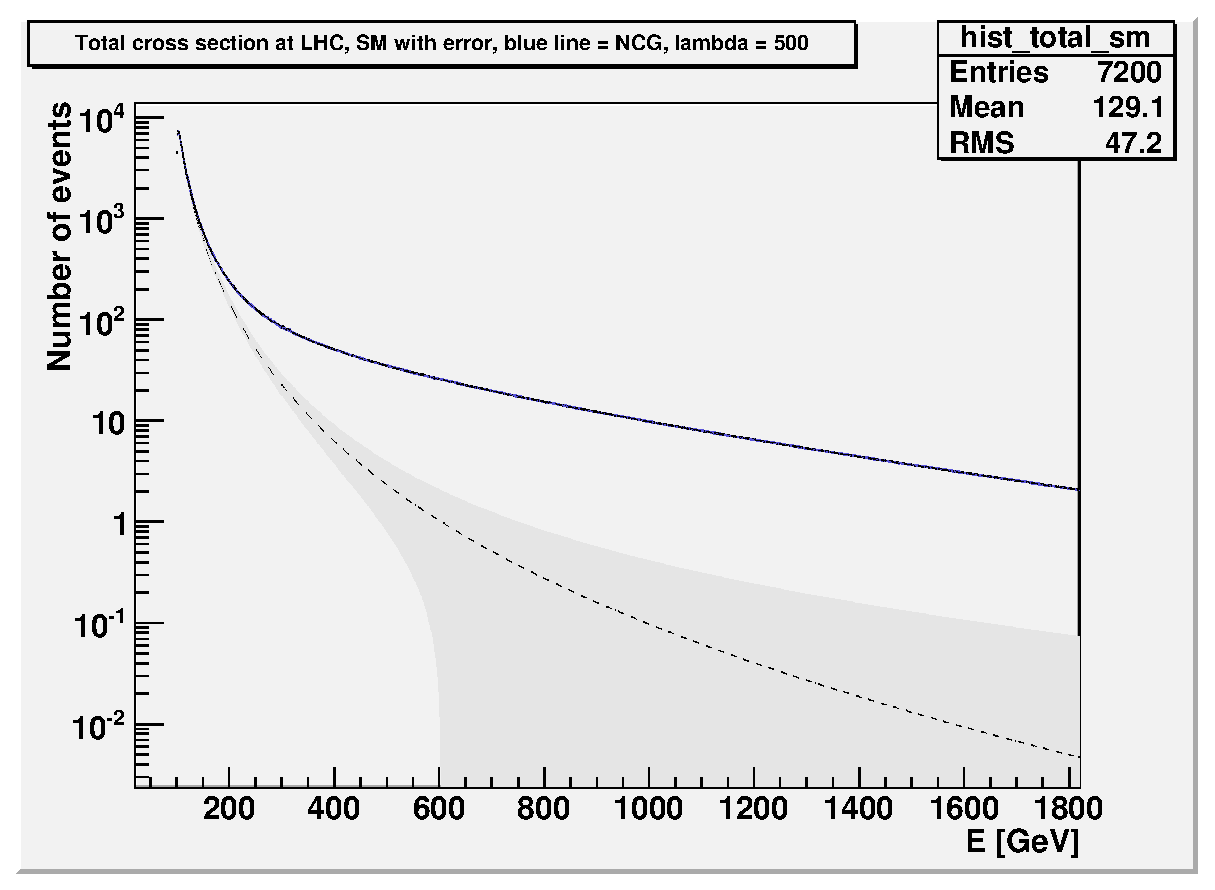
\includegraphics[scale=0.35]{./images/L500r139.eps}
	\end{minipage}
	%\hspace{0.5cm}
	\begin{minipage}[b]{0.475\linewidth}
    \centering
	  \includegraphics[scale=0.35]{./images/L900r139.eps}
	\end{minipage}
	\\ \vspace{0.5cm}
	\begin{minipage}[b]{0.475\linewidth}
    \centering
	  \includegraphics[scale=0.35]{./images/L1500r139.eps}
	\end{minipage}
	%\hspace{0.5cm}
	\begin{minipage}[b]{0.475\linewidth}
    \centering
	  \includegraphics[scale=0.35]{./images/L2000r139.eps}
	\end{minipage}
		\caption{Predicted number of $pp \rightarrow Z/ \gamma \rightarrow \mu \bar \mu$ events at LHC running with a luminosity of $L=10 \textrm{ fb}^{-1}$ for one year. The grey line shows number of events as predicted by the SM with error $1.64\sigma = 1.64\sqrt{N}$, where $N$ is the number of events in the given bin. The blue line represent number of events as predicted by NCG for the given value of $\Lambda$. All interference terms and possible NCG contributions from $\gamma gg$ vertices have been ignored.} \label{fig:lambdaplot}
\end{figure}
We have made histograms showing the expected number of muon-pair production events at LHC with integrated luminosity of $10 \textrm{ fb}^{-1}$ running for 1 year.\footnote{To get from cross section to $N$ we simply multiply the histograms by $10^4$ fb $\cdot$ pb$^{-1}$.} The distributions are made using leading order diagrams in CompHEP (Figures \ref{fig:feyn:parton_qq} and \ref{fig:feyn:parton_gg}) for the process $pp \rightarrow Z \rightarrow \mu \bar \mu$. All interference terms have been ignored. As have contributions from diagrams involving vertices $\gamma gg$. Four different plots are made for different values of $\Lambda$. The statistical error, $1.64\sqrt{N}$, where $N$ is the number of events in the given bin, is shown by the gray band for the ordinary SM data. Cross sections with contributions from NCG are shown as a blue line. Note that we have made all plots up to an energy of $\sqrt{s} \sim 1800$ GeV, even though we made an approximation, in the zero-range interaction scheme, valid only for $\sqrt{s} \ll \Lambda$.\footnote{See the derivation in section \ref{sec:derivcrosssection}.} In the complete description we would naturally observe a peak in the NCG cross section around the value of $\Lambda$, in analogy to the $Z$. Our approximation ignores this behavior completely and instead we obtain an extrapolation of the low energy behavior for $\sqrt{s} \ll \Lambda$. This extrapolation can still be instructive to look at even for high energies where our approximation no longer holds.

Assuming that NCG holds true and for $\Lambda < 900$ GeV we should be able to detect a significant increase in the number of events (CL > 95\%). For $\Lambda > 900$ GeV the additional events coming from NCG vertices are lost due statistical uncertainty in the data.

% % % % % % % % % % % % % % CONCLUSION % % % % % % % % % % % % % % % % %

\include{conclusions}

% % % % % % % % % % % % % % % BIBTEX % % % % % % % % % % % % % % % % % %

\clearpage

\bibliographystyle{plain}

% The standard styles distributed with BIBTeX
% alpha	 Sorted alphabetically. Labels are formed from name of author and year of publication with entry labels like "Knu66" formed from the author's name and the year of publication.
% plain	Standard style for producing bibliographies that are sorted alphabetically by author and labeled with numbers.
% unsrt	 Like `plain', but entries are in order of citation. Standard style for producing bibliographies that are labeled with numbers and with entries that appear in the order of their first citation.
% abbrv	 Like `plain', but more compact labels. Standard style for producing bibliographies that are sorted alphabetically by author and labeled with numbers. Author names, month names and journal names are abbreviated.

\bibliography{ncg_citations}		% Navn paa BibTex -filen

\clearpage

%\pagenumbering{Alph}

% % % % % % % % % % % % % % APPENDICES % % % % % % % % % % % % % % % % %

\section{Appendix A}

Lidt om tensor notation og Einstein summation. Eller skal vi droppe det!?

\clearpage


\section{Appendix B}
\subsection{Cross Sections}


\clearpage


% % % % % % % % % % % % % % SLUT PRUT % % % % % % % % % % % % % % % % % %

\end{document}
